\chapter{Model Development Lifecycle}
\label{ch:model_development}

\section*{Learning Objectives}

By the end of this chapter, you will be able to:

\begin{itemize}
    \item Design systematic model selection strategies based on problem constraints and requirements
    \item Implement iterative model development workflows with proper versioning and tracking
    \item Apply model interpretability techniques using SHAP, LIME, and other explainability methods
    \item Design robust cross-validation strategies and evaluate models comprehensively
    \item Optimize hyperparameters efficiently using Bayesian optimization and other advanced methods
    \item Debug and diagnose model issues using systematic diagnostic frameworks
    \item Balance model complexity, performance, and interpretability for production systems
\end{itemize}

\section{Introduction}

Model development in production ML systems differs significantly from exploratory data science. While research projects may focus on achieving state-of-the-art performance, production models must balance accuracy, latency, interpretability, maintainability, and operational costs.

The model development lifecycle encompasses the systematic process of selecting, training, evaluating, and refining models. This chapter presents production-grade patterns and practices for each stage of this lifecycle, from initial model selection through final deployment readiness.

\subsection{Production Model Requirements}

Production models must satisfy multiple, often competing requirements:

\begin{table}[h]
\centering
\caption{Production Model Trade-offs}
\label{tab:model_tradeoffs}
\begin{tabular}{|l|l|l|}
\hline
\textbf{Requirement} & \textbf{Priority Factors} & \textbf{Trade-offs} \\
\hline
Accuracy & Business impact, SLA requirements & Training time, complexity \\
Latency & User experience, real-time constraints & Model size, accuracy \\
Interpretability & Regulatory, trust, debugging & Model complexity \\
Robustness & Data drift, edge cases & Training data requirements \\
Maintainability & Team skills, documentation & Development velocity \\
Cost & Infrastructure, training, serving & Performance optimization \\
\hline
\end{tabular}
\end{table}

\subsection{Development Lifecycle Stages}

The model development lifecycle follows a structured progression:

\begin{enumerate}
    \item \textbf{Problem Formulation:} Define success metrics, constraints, and requirements
    \item \textbf{Model Selection:} Choose appropriate model families and architectures
    \item \textbf{Baseline Development:} Establish simple, interpretable baselines
    \item \textbf{Iterative Improvement:} Systematically enhance model performance
    \item \textbf{Evaluation and Validation:} Comprehensive assessment across multiple dimensions
    \item \textbf{Interpretability Analysis:} Understand model behavior and predictions
    \item \textbf{Debugging and Diagnosis:} Identify and resolve model issues
    \item \textbf{Production Readiness:} Optimize for deployment and operation
\end{enumerate}

\section{Model Selection Strategy}

Model selection is the process of choosing the most appropriate model family and architecture for a given problem. This decision significantly impacts development velocity, performance, and operational costs.

\subsection{Model Selection Framework}

A systematic approach to model selection considers problem characteristics, constraints, and requirements:

\begin{lstlisting}[style=python, caption={Automated Model Selection Framework}]
from typing import Dict, List, Any, Optional, Callable
from dataclasses import dataclass
import pandas as pd
import numpy as np
from sklearn.base import BaseEstimator
from sklearn.linear_model import LogisticRegression, Ridge
from sklearn.ensemble import RandomForestClassifier, GradientBoostingClassifier
from sklearn.svm import SVC
from sklearn.neural_network import MLPClassifier
from sklearn.model_selection import cross_val_score
from sklearn.metrics import make_scorer
import logging
import time

@dataclass
class ModelConstraints:
    """Constraints for model selection."""
    max_training_time_seconds: Optional[float] = None
    max_inference_latency_ms: Optional[float] = None
    max_model_size_mb: Optional[float] = None
    min_accuracy: Optional[float] = None
    require_interpretability: bool = False
    require_probabilistic: bool = False
    available_memory_gb: float = 16.0

@dataclass
class ModelCandidate:
    """Model candidate with metadata."""
    name: str
    model: BaseEstimator
    interpretability_score: int  # 1-10, 10=most interpretable
    typical_latency_ms: float
    typical_size_mb: float
    requires_scaling: bool
    requires_encoding: bool
    hyperparameter_space: Dict[str, Any]

class ModelSelector:
    """
    Automated model selection based on problem characteristics and constraints.

    This class implements a systematic approach to model selection that:
    1. Filters candidates based on hard constraints
    2. Benchmarks remaining candidates
    3. Selects the best model based on multi-objective optimization
    """

    def __init__(
        self,
        problem_type: str = "classification",
        constraints: Optional[ModelConstraints] = None,
        optimization_metric: str = "accuracy",
        cv_folds: int = 5,
        random_state: int = 42
    ):
        """
        Initialize model selector.

        Args:
            problem_type: 'classification' or 'regression'
            constraints: Model constraints
            optimization_metric: Metric to optimize
            cv_folds: Number of cross-validation folds
            random_state: Random seed for reproducibility
        """
        self.problem_type = problem_type
        self.constraints = constraints or ModelConstraints()
        self.optimization_metric = optimization_metric
        self.cv_folds = cv_folds
        self.random_state = random_state
        self.logger = logging.getLogger(__name__)

        # Initialize model candidates
        self.candidates = self._initialize_candidates()

    def _initialize_candidates(self) -> List[ModelCandidate]:
        """Initialize model candidates based on problem type."""
        if self.problem_type == "classification":
            return [
                ModelCandidate(
                    name="Logistic Regression",
                    model=LogisticRegression(random_state=self.random_state, max_iter=1000),
                    interpretability_score=9,
                    typical_latency_ms=1.0,
                    typical_size_mb=0.1,
                    requires_scaling=True,
                    requires_encoding=True,
                    hyperparameter_space={
                        'C': [0.001, 0.01, 0.1, 1.0, 10.0],
                        'penalty': ['l1', 'l2'],
                        'solver': ['liblinear', 'saga']
                    }
                ),
                ModelCandidate(
                    name="Random Forest",
                    model=RandomForestClassifier(random_state=self.random_state),
                    interpretability_score=6,
                    typical_latency_ms=10.0,
                    typical_size_mb=50.0,
                    requires_scaling=False,
                    requires_encoding=True,
                    hyperparameter_space={
                        'n_estimators': [50, 100, 200],
                        'max_depth': [5, 10, 20, None],
                        'min_samples_split': [2, 5, 10]
                    }
                ),
                ModelCandidate(
                    name="Gradient Boosting",
                    model=GradientBoostingClassifier(random_state=self.random_state),
                    interpretability_score=5,
                    typical_latency_ms=15.0,
                    typical_size_mb=30.0,
                    requires_scaling=False,
                    requires_encoding=True,
                    hyperparameter_space={
                        'n_estimators': [50, 100, 200],
                        'learning_rate': [0.01, 0.1, 0.3],
                        'max_depth': [3, 5, 7]
                    }
                ),
                ModelCandidate(
                    name="SVM",
                    model=SVC(random_state=self.random_state, probability=True),
                    interpretability_score=4,
                    typical_latency_ms=20.0,
                    typical_size_mb=10.0,
                    requires_scaling=True,
                    requires_encoding=True,
                    hyperparameter_space={
                        'C': [0.1, 1.0, 10.0],
                        'kernel': ['rbf', 'linear'],
                        'gamma': ['scale', 'auto']
                    }
                ),
                ModelCandidate(
                    name="Neural Network",
                    model=MLPClassifier(random_state=self.random_state, max_iter=1000),
                    interpretability_score=2,
                    typical_latency_ms=5.0,
                    typical_size_mb=20.0,
                    requires_scaling=True,
                    requires_encoding=True,
                    hyperparameter_space={
                        'hidden_layer_sizes': [(50,), (100,), (100, 50)],
                        'activation': ['relu', 'tanh'],
                        'alpha': [0.0001, 0.001, 0.01]
                    }
                )
            ]
        else:  # regression
            return [
                ModelCandidate(
                    name="Ridge Regression",
                    model=Ridge(random_state=self.random_state),
                    interpretability_score=9,
                    typical_latency_ms=1.0,
                    typical_size_mb=0.1,
                    requires_scaling=True,
                    requires_encoding=True,
                    hyperparameter_space={
                        'alpha': [0.001, 0.01, 0.1, 1.0, 10.0]
                    }
                ),
                # Additional regression models...
            ]

    def filter_candidates(self) -> List[ModelCandidate]:
        """Filter candidates based on hard constraints."""
        filtered = []

        for candidate in self.candidates:
            # Check interpretability requirement
            if self.constraints.require_interpretability and candidate.interpretability_score < 7:
                self.logger.info(f"Filtered {candidate.name}: interpretability too low")
                continue

            # Check latency constraint
            if (self.constraints.max_inference_latency_ms and
                candidate.typical_latency_ms > self.constraints.max_inference_latency_ms):
                self.logger.info(f"Filtered {candidate.name}: latency too high")
                continue

            # Check model size constraint
            if (self.constraints.max_model_size_mb and
                candidate.typical_size_mb > self.constraints.max_model_size_mb):
                self.logger.info(f"Filtered {candidate.name}: model size too large")
                continue

            # Check probabilistic requirement
            if self.constraints.require_probabilistic:
                if not hasattr(candidate.model, 'predict_proba'):
                    self.logger.info(f"Filtered {candidate.name}: no probability support")
                    continue

            filtered.append(candidate)

        self.logger.info(f"Filtered to {len(filtered)} candidates from {len(self.candidates)}")
        return filtered

    def benchmark_candidates(
        self,
        X: pd.DataFrame,
        y: pd.Series,
        candidates: List[ModelCandidate]
    ) -> pd.DataFrame:
        """
        Benchmark model candidates using cross-validation.

        Args:
            X: Training features
            y: Training target
            candidates: List of model candidates to benchmark

        Returns:
            DataFrame with benchmark results
        """
        results = []

        for candidate in candidates:
            self.logger.info(f"Benchmarking {candidate.name}...")

            # Measure training time
            start_time = time.time()

            try:
                # Cross-validation
                scores = cross_val_score(
                    candidate.model,
                    X,
                    y,
                    cv=self.cv_folds,
                    scoring=self.optimization_metric,
                    n_jobs=-1
                )

                training_time = time.time() - start_time

                # Check training time constraint
                if (self.constraints.max_training_time_seconds and
                    training_time > self.constraints.max_training_time_seconds):
                    self.logger.warning(
                        f"{candidate.name} exceeded training time limit: "
                        f"{training_time:.2f}s > {self.constraints.max_training_time_seconds}s"
                    )
                    continue

                # Check minimum accuracy constraint
                mean_score = scores.mean()
                if (self.constraints.min_accuracy and
                    mean_score < self.constraints.min_accuracy):
                    self.logger.warning(
                        f"{candidate.name} below minimum accuracy: "
                        f"{mean_score:.4f} < {self.constraints.min_accuracy}"
                    )
                    continue

                results.append({
                    'model_name': candidate.name,
                    'mean_score': mean_score,
                    'std_score': scores.std(),
                    'training_time_seconds': training_time,
                    'interpretability_score': candidate.interpretability_score,
                    'typical_latency_ms': candidate.typical_latency_ms,
                    'typical_size_mb': candidate.typical_size_mb,
                    'requires_scaling': candidate.requires_scaling,
                    'requires_encoding': candidate.requires_encoding
                })

            except Exception as e:
                self.logger.error(f"Error benchmarking {candidate.name}: {e}")
                continue

        df_results = pd.DataFrame(results)
        return df_results.sort_values('mean_score', ascending=False)

    def select_best_model(
        self,
        benchmark_results: pd.DataFrame,
        interpretability_weight: float = 0.2,
        latency_weight: float = 0.3,
        accuracy_weight: float = 0.5
    ) -> Dict[str, Any]:
        """
        Select best model using multi-objective optimization.

        Args:
            benchmark_results: Results from benchmarking
            interpretability_weight: Weight for interpretability (0-1)
            latency_weight: Weight for latency (0-1)
            accuracy_weight: Weight for accuracy (0-1)

        Returns:
            Dictionary with selected model information
        """
        # Normalize scores
        df = benchmark_results.copy()
        df['norm_accuracy'] = (df['mean_score'] - df['mean_score'].min()) / \
                              (df['mean_score'].max() - df['mean_score'].min())
        df['norm_interpretability'] = df['interpretability_score'] / 10.0
        df['norm_latency'] = 1.0 - (df['typical_latency_ms'] - df['typical_latency_ms'].min()) / \
                                   (df['typical_latency_ms'].max() - df['typical_latency_ms'].min())

        # Calculate composite score
        df['composite_score'] = (
            accuracy_weight * df['norm_accuracy'] +
            interpretability_weight * df['norm_interpretability'] +
            latency_weight * df['norm_latency']
        )

        # Select best
        best_idx = df['composite_score'].idxmax()
        best_model = df.loc[best_idx]

        self.logger.info(f"Selected model: {best_model['model_name']}")
        self.logger.info(f"  Accuracy: {best_model['mean_score']:.4f}")
        self.logger.info(f"  Interpretability: {best_model['interpretability_score']}/10")
        self.logger.info(f"  Latency: {best_model['typical_latency_ms']:.2f}ms")

        return {
            'model_name': best_model['model_name'],
            'mean_score': best_model['mean_score'],
            'std_score': best_model['std_score'],
            'composite_score': best_model['composite_score'],
            'training_time_seconds': best_model['training_time_seconds'],
            'all_results': df.to_dict('records')
        }

    def select(
        self,
        X: pd.DataFrame,
        y: pd.Series,
        interpretability_weight: float = 0.2,
        latency_weight: float = 0.3,
        accuracy_weight: float = 0.5
    ) -> Dict[str, Any]:
        """
        Complete model selection pipeline.

        Args:
            X: Training features
            y: Training target
            interpretability_weight: Weight for interpretability
            latency_weight: Weight for latency
            accuracy_weight: Weight for accuracy

        Returns:
            Dictionary with selected model information
        """
        # Filter candidates
        filtered_candidates = self.filter_candidates()

        if not filtered_candidates:
            raise ValueError("No candidates passed constraint filtering")

        # Benchmark candidates
        benchmark_results = self.benchmark_candidates(X, y, filtered_candidates)

        if benchmark_results.empty:
            raise ValueError("No candidates passed benchmarking")

        # Select best model
        selection_result = self.select_best_model(
            benchmark_results,
            interpretability_weight,
            latency_weight,
            accuracy_weight
        )

        return selection_result

# Example usage
if __name__ == "__main__":
    from sklearn.datasets import make_classification

    # Generate sample data
    X, y = make_classification(
        n_samples=10000,
        n_features=20,
        n_informative=15,
        n_redundant=5,
        random_state=42
    )
    X = pd.DataFrame(X, columns=[f'feature_{i}' for i in range(20)])
    y = pd.Series(y, name='target')

    # Define constraints
    constraints = ModelConstraints(
        max_training_time_seconds=60.0,
        max_inference_latency_ms=50.0,
        max_model_size_mb=100.0,
        min_accuracy=0.75,
        require_interpretability=False,
        require_probabilistic=True
    )

    # Select model
    selector = ModelSelector(
        problem_type="classification",
        constraints=constraints,
        optimization_metric="f1_weighted"
    )

    result = selector.select(
        X, y,
        interpretability_weight=0.3,
        latency_weight=0.2,
        accuracy_weight=0.5
    )

    print(f"Selected model: {result['model_name']}")
    print(f"F1 Score: {result['mean_score']:.4f} +/- {result['std_score']:.4f}")
\end{lstlisting}

\subsection{Model Selection Decision Tree}

The following decision tree provides guidance for model selection based on problem characteristics:

\begin{figure}[h]
\centering
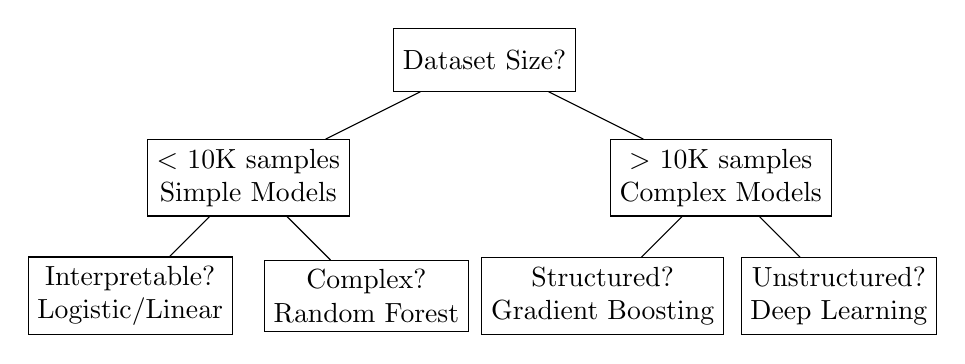
\begin{tikzpicture}[
    level distance=1.5cm,
    level 1/.style={sibling distance=6cm},
    level 2/.style={sibling distance=3cm},
    every node/.style={rectangle, draw, align=center, minimum height=0.8cm}
]
\node {Dataset Size?}
    child {node {$<$ 10K samples\\Simple Models}
        child {node {Interpretable?\\Logistic/Linear}}
        child {node {Complex?\\Random Forest}}
    }
    child {node {$>$ 10K samples\\Complex Models}
        child {node {Structured?\\Gradient Boosting}}
        child {node {Unstructured?\\Deep Learning}}
    };
\end{tikzpicture}
\caption{Model Selection Decision Tree}
\label{fig:model_selection_tree}
\end{figure}

\section{Iterative Model Development}

Iterative model development is a systematic approach to progressively improving model performance while maintaining reproducibility and tracking improvements.

\subsection{Progressive Improvement Framework}

\begin{lstlisting}[style=python, caption={Iterative Model Development Framework}]
from typing import Dict, List, Optional, Tuple, Callable
from dataclasses import dataclass, field
from datetime import datetime
import json
import hashlib
from pathlib import Path
import mlflow
import pandas as pd
import numpy as np
from sklearn.base import clone
from sklearn.metrics import classification_report, confusion_matrix
import matplotlib.pyplot as plt
import seaborn as sns

@dataclass
class ModelVersion:
    """Represents a version of a model in the development lifecycle."""
    version_id: str
    version_number: int
    timestamp: datetime
    model: BaseEstimator
    metrics: Dict[str, float]
    hyperparameters: Dict[str, Any]
    feature_set: List[str]
    description: str
    parent_version: Optional[str] = None
    git_commit: Optional[str] = None

    def to_dict(self) -> Dict[str, Any]:
        """Convert to dictionary for serialization."""
        return {
            'version_id': self.version_id,
            'version_number': self.version_number,
            'timestamp': self.timestamp.isoformat(),
            'metrics': self.metrics,
            'hyperparameters': self.hyperparameters,
            'feature_set': self.feature_set,
            'description': self.description,
            'parent_version': self.parent_version,
            'git_commit': self.git_commit
        }

class IterativeModelDeveloper:
    """
    Framework for iterative model development with version control.

    Features:
    - Automatic version tracking
    - Performance comparison across versions
    - Feature set evolution tracking
    - Experiment lineage
    - Automatic rollback to best version
    """

    def __init__(
        self,
        project_name: str,
        base_model: BaseEstimator,
        optimization_metric: str = "f1_weighted",
        experiment_dir: str = "./experiments",
        mlflow_tracking_uri: Optional[str] = None
    ):
        """
        Initialize iterative model developer.

        Args:
            project_name: Name of the project
            base_model: Base model to iterate on
            optimization_metric: Metric to optimize
            experiment_dir: Directory for experiment artifacts
            mlflow_tracking_uri: MLflow tracking server URI
        """
        self.project_name = project_name
        self.base_model = base_model
        self.optimization_metric = optimization_metric
        self.experiment_dir = Path(experiment_dir)
        self.experiment_dir.mkdir(parents=True, exist_ok=True)

        # MLflow setup
        if mlflow_tracking_uri:
            mlflow.set_tracking_uri(mlflow_tracking_uri)
        mlflow.set_experiment(project_name)

        # Version tracking
        self.versions: List[ModelVersion] = []
        self.current_version: Optional[ModelVersion] = None
        self.best_version: Optional[ModelVersion] = None

        self.logger = logging.getLogger(__name__)

    def _generate_version_id(self, description: str) -> str:
        """Generate unique version ID."""
        content = f"{description}_{datetime.now().isoformat()}"
        return hashlib.sha256(content.encode()).hexdigest()[:12]

    def _get_git_commit(self) -> Optional[str]:
        """Get current git commit hash."""
        try:
            import subprocess
            result = subprocess.run(
                ['git', 'rev-parse', 'HEAD'],
                capture_output=True,
                text=True,
                check=True
            )
            return result.stdout.strip()
        except:
            return None

    def create_version(
        self,
        model: BaseEstimator,
        X_train: pd.DataFrame,
        y_train: pd.Series,
        X_val: pd.DataFrame,
        y_val: pd.Series,
        description: str,
        hyperparameters: Optional[Dict[str, Any]] = None
    ) -> ModelVersion:
        """
        Create a new model version.

        Args:
            model: Trained model
            X_train: Training features
            y_train: Training target
            X_val: Validation features
            y_val: Validation target
            description: Description of changes
            hyperparameters: Model hyperparameters

        Returns:
            Created model version
        """
        version_number = len(self.versions) + 1
        version_id = self._generate_version_id(description)

        with mlflow.start_run(run_name=f"v{version_number}_{version_id}"):
            # Log parameters
            if hyperparameters:
                mlflow.log_params(hyperparameters)

            # Evaluate on training set
            train_predictions = model.predict(X_train)
            train_metrics = self._calculate_metrics(y_train, train_predictions, prefix="train_")

            # Evaluate on validation set
            val_predictions = model.predict(X_val)
            val_metrics = self._calculate_metrics(y_val, val_predictions, prefix="val_")

            # Combine metrics
            all_metrics = {**train_metrics, **val_metrics}
            mlflow.log_metrics(all_metrics)

            # Log model
            mlflow.sklearn.log_model(model, "model")

            # Log feature importance if available
            if hasattr(model, 'feature_importances_'):
                self._log_feature_importance(model, X_train.columns, version_id)

            # Log confusion matrix
            self._log_confusion_matrix(y_val, val_predictions, version_id)

            # Create version
            version = ModelVersion(
                version_id=version_id,
                version_number=version_number,
                timestamp=datetime.now(),
                model=model,
                metrics=all_metrics,
                hyperparameters=hyperparameters or {},
                feature_set=list(X_train.columns),
                description=description,
                parent_version=self.current_version.version_id if self.current_version else None,
                git_commit=self._get_git_commit()
            )

            # Update tracking
            self.versions.append(version)
            self.current_version = version

            # Update best version
            val_metric = val_metrics.get(f"val_{self.optimization_metric}", 0)
            if self.best_version is None:
                self.best_version = version
            else:
                best_metric = self.best_version.metrics.get(f"val_{self.optimization_metric}", 0)
                if val_metric > best_metric:
                    self.best_version = version
                    self.logger.info(f"New best model: v{version_number} ({val_metric:.4f})")

            # Save version metadata
            self._save_version_metadata(version)

            mlflow.log_artifact(str(self.experiment_dir / f"version_{version_id}.json"))

        return version

    def _calculate_metrics(
        self,
        y_true: np.ndarray,
        y_pred: np.ndarray,
        prefix: str = ""
    ) -> Dict[str, float]:
        """Calculate classification metrics."""
        from sklearn.metrics import (
            accuracy_score, precision_score, recall_score,
            f1_score, roc_auc_score
        )

        metrics = {
            f"{prefix}accuracy": accuracy_score(y_true, y_pred),
            f"{prefix}precision": precision_score(y_true, y_pred, average='weighted', zero_division=0),
            f"{prefix}recall": recall_score(y_true, y_pred, average='weighted', zero_division=0),
            f"{prefix}f1_weighted": f1_score(y_true, y_pred, average='weighted', zero_division=0),
        }

        return metrics

    def _log_feature_importance(
        self,
        model: BaseEstimator,
        feature_names: List[str],
        version_id: str
    ):
        """Log feature importance plot."""
        importances = model.feature_importances_
        indices = np.argsort(importances)[::-1][:20]  # Top 20

        plt.figure(figsize=(10, 6))
        plt.title("Feature Importance")
        plt.bar(range(len(indices)), importances[indices])
        plt.xticks(range(len(indices)), [feature_names[i] for i in indices], rotation=45, ha='right')
        plt.tight_layout()

        plot_path = self.experiment_dir / f"feature_importance_{version_id}.png"
        plt.savefig(plot_path)
        mlflow.log_artifact(str(plot_path))
        plt.close()

    def _log_confusion_matrix(
        self,
        y_true: np.ndarray,
        y_pred: np.ndarray,
        version_id: str
    ):
        """Log confusion matrix plot."""
        cm = confusion_matrix(y_true, y_pred)

        plt.figure(figsize=(8, 6))
        sns.heatmap(cm, annot=True, fmt='d', cmap='Blues')
        plt.title("Confusion Matrix")
        plt.ylabel('True Label')
        plt.xlabel('Predicted Label')
        plt.tight_layout()

        plot_path = self.experiment_dir / f"confusion_matrix_{version_id}.png"
        plt.savefig(plot_path)
        mlflow.log_artifact(str(plot_path))
        plt.close()

    def _save_version_metadata(self, version: ModelVersion):
        """Save version metadata to JSON."""
        metadata_path = self.experiment_dir / f"version_{version.version_id}.json"
        with open(metadata_path, 'w') as f:
            json.dump(version.to_dict(), f, indent=2)

    def compare_versions(
        self,
        version_ids: Optional[List[str]] = None,
        top_n: int = 5
    ) -> pd.DataFrame:
        """
        Compare model versions.

        Args:
            version_ids: Specific versions to compare (None = all)
            top_n: Number of top versions to show

        Returns:
            DataFrame with version comparison
        """
        if version_ids:
            versions = [v for v in self.versions if v.version_id in version_ids]
        else:
            versions = self.versions

        # Sort by validation metric
        versions = sorted(
            versions,
            key=lambda v: v.metrics.get(f"val_{self.optimization_metric}", 0),
            reverse=True
        )[:top_n]

        comparison_data = []
        for v in versions:
            comparison_data.append({
                'Version': f"v{v.version_number}",
                'ID': v.version_id[:8],
                'Description': v.description,
                'Val Metric': v.metrics.get(f"val_{self.optimization_metric}", 0),
                'Train Metric': v.metrics.get(f"train_{self.optimization_metric}", 0),
                'Timestamp': v.timestamp.strftime('%Y-%m-%d %H:%M'),
                'Features': len(v.feature_set)
            })

        df = pd.DataFrame(comparison_data)
        return df

    def rollback_to_best(self) -> ModelVersion:
        """Rollback to best performing version."""
        if self.best_version is None:
            raise ValueError("No versions available")

        self.current_version = self.best_version
        self.logger.info(
            f"Rolled back to v{self.best_version.version_number} "
            f"({self.best_version.version_id[:8]})"
        )
        return self.best_version

    def get_improvement_trajectory(self) -> pd.DataFrame:
        """Get improvement trajectory over versions."""
        data = []
        for v in self.versions:
            data.append({
                'version_number': v.version_number,
                'timestamp': v.timestamp,
                'val_metric': v.metrics.get(f"val_{self.optimization_metric}", 0),
                'train_metric': v.metrics.get(f"train_{self.optimization_metric}", 0),
                'description': v.description
            })

        df = pd.DataFrame(data)
        return df.sort_values('version_number')

    def plot_improvement_trajectory(self):
        """Plot improvement trajectory."""
        df = self.get_improvement_trajectory()

        plt.figure(figsize=(12, 6))
        plt.plot(df['version_number'], df['val_metric'], marker='o', label='Validation')
        plt.plot(df['version_number'], df['train_metric'], marker='s', label='Training', alpha=0.6)
        plt.xlabel('Version Number')
        plt.ylabel(self.optimization_metric.capitalize())
        plt.title('Model Improvement Trajectory')
        plt.legend()
        plt.grid(True, alpha=0.3)
        plt.tight_layout()

        plot_path = self.experiment_dir / "improvement_trajectory.png"
        plt.savefig(plot_path)
        plt.close()

        return plot_path

# Example usage
if __name__ == "__main__":
    from sklearn.datasets import make_classification
    from sklearn.model_selection import train_test_split
    from sklearn.ensemble import RandomForestClassifier

    # Generate sample data
    X, y = make_classification(n_samples=5000, n_features=20, n_informative=15, random_state=42)
    X = pd.DataFrame(X, columns=[f'feature_{i}' for i in range(20)])
    y = pd.Series(y)

    # Split data
    X_train, X_temp, y_train, y_temp = train_test_split(X, y, test_size=0.3, random_state=42)
    X_val, X_test, y_val, y_test = train_test_split(X_temp, y_temp, test_size=0.5, random_state=42)

    # Initialize developer
    developer = IterativeModelDeveloper(
        project_name="iterative_development_example",
        base_model=RandomForestClassifier(random_state=42),
        optimization_metric="f1_weighted"
    )

    # Version 1: Baseline
    model_v1 = RandomForestClassifier(n_estimators=50, max_depth=5, random_state=42)
    model_v1.fit(X_train, y_train)
    v1 = developer.create_version(
        model_v1, X_train, y_train, X_val, y_val,
        description="Baseline model with default hyperparameters",
        hyperparameters={'n_estimators': 50, 'max_depth': 5}
    )

    # Version 2: Increase depth
    model_v2 = RandomForestClassifier(n_estimators=50, max_depth=10, random_state=42)
    model_v2.fit(X_train, y_train)
    v2 = developer.create_version(
        model_v2, X_train, y_train, X_val, y_val,
        description="Increased max_depth to 10",
        hyperparameters={'n_estimators': 50, 'max_depth': 10}
    )

    # Version 3: Increase estimators
    model_v3 = RandomForestClassifier(n_estimators=100, max_depth=10, random_state=42)
    model_v3.fit(X_train, y_train)
    v3 = developer.create_version(
        model_v3, X_train, y_train, X_val, y_val,
        description="Increased n_estimators to 100",
        hyperparameters={'n_estimators': 100, 'max_depth': 10}
    )

    # Compare versions
    print("\nVersion Comparison:")
    print(developer.compare_versions())

    # Plot trajectory
    developer.plot_improvement_trajectory()

    # Get best model
    print(f"\nBest model: v{developer.best_version.version_number}")
\end{lstlisting}

\section{Model Interpretability and Explainability}

Model interpretability is critical for production ML systems, enabling debugging, trust, regulatory compliance, and stakeholder communication.

\subsection{Interpretability Spectrum}

Different models offer different levels of interpretability:

\begin{table}[h]
\centering
\caption{Model Interpretability Levels}
\label{tab:interpretability_levels}
\begin{tabular}{|l|l|l|l|}
\hline
\textbf{Level} & \textbf{Models} & \textbf{Techniques} & \textbf{Use Cases} \\
\hline
High & Linear, Decision Trees & Coefficients, rules & Regulated industries \\
Medium & Random Forest, GBM & Feature importance & Most applications \\
Low & Neural Networks, SVM & SHAP, LIME & Complex patterns \\
\hline
\end{tabular}
\end{table}

\subsection{SHAP and LIME Implementation}

\begin{lstlisting}[style=python, caption={Model Interpretability Framework with SHAP and LIME}]
from typing import Dict, List, Optional, Union, Any
import pandas as pd
import numpy as np
import matplotlib.pyplot as plt
import seaborn as sns
from sklearn.base import BaseEstimator
import shap
from lime import lime_tabular
from lime.lime_tabular import LimeTabularExplainer
import logging

class ModelInterpreter:
    """
    Comprehensive model interpretability framework.

    Provides multiple interpretation techniques:
    - SHAP (SHapley Additive exPlanations)
    - LIME (Local Interpretable Model-agnostic Explanations)
    - Feature importance
    - Partial dependence plots
    - Individual prediction explanations
    """

    def __init__(
        self,
        model: BaseEstimator,
        X_train: pd.DataFrame,
        feature_names: Optional[List[str]] = None,
        class_names: Optional[List[str]] = None,
        categorical_features: Optional[List[str]] = None
    ):
        """
        Initialize model interpreter.

        Args:
            model: Trained model
            X_train: Training data for background distribution
            feature_names: Names of features
            class_names: Names of classes (for classification)
            categorical_features: Names of categorical features
        """
        self.model = model
        self.X_train = X_train
        self.feature_names = feature_names or list(X_train.columns)
        self.class_names = class_names
        self.categorical_features = categorical_features or []
        self.logger = logging.getLogger(__name__)

        # Initialize SHAP explainer
        self._init_shap_explainer()

        # Initialize LIME explainer
        self._init_lime_explainer()

    def _init_shap_explainer(self):
        """Initialize SHAP explainer based on model type."""
        try:
            # Try TreeExplainer for tree-based models (faster)
            if hasattr(self.model, 'tree_'):
                self.shap_explainer = shap.TreeExplainer(self.model)
                self.logger.info("Using SHAP TreeExplainer")
            elif hasattr(self.model, 'estimators_'):
                self.shap_explainer = shap.TreeExplainer(self.model)
                self.logger.info("Using SHAP TreeExplainer for ensemble")
            else:
                # Use KernelExplainer for model-agnostic approach
                # Sample background data for efficiency
                background = shap.sample(self.X_train, min(100, len(self.X_train)))
                self.shap_explainer = shap.KernelExplainer(
                    self.model.predict_proba if hasattr(self.model, 'predict_proba') else self.model.predict,
                    background
                )
                self.logger.info("Using SHAP KernelExplainer")
        except Exception as e:
            self.logger.warning(f"SHAP explainer initialization failed: {e}")
            self.shap_explainer = None

    def _init_lime_explainer(self):
        """Initialize LIME explainer."""
        try:
            # Identify categorical feature indices
            categorical_indices = [
                self.feature_names.index(f) for f in self.categorical_features
                if f in self.feature_names
            ]

            self.lime_explainer = LimeTabularExplainer(
                training_data=self.X_train.values,
                feature_names=self.feature_names,
                class_names=self.class_names,
                categorical_features=categorical_indices,
                mode='classification' if hasattr(self.model, 'predict_proba') else 'regression'
            )
            self.logger.info("LIME explainer initialized")
        except Exception as e:
            self.logger.warning(f"LIME explainer initialization failed: {e}")
            self.lime_explainer = None

    def explain_global_shap(
        self,
        X: pd.DataFrame,
        max_display: int = 20,
        plot: bool = True
    ) -> Optional[np.ndarray]:
        """
        Generate global SHAP explanations.

        Args:
            X: Data to explain
            max_display: Maximum features to display
            plot: Whether to generate plots

        Returns:
            SHAP values array
        """
        if self.shap_explainer is None:
            self.logger.warning("SHAP explainer not available")
            return None

        # Calculate SHAP values
        shap_values = self.shap_explainer.shap_values(X)

        if plot:
            # Summary plot
            plt.figure(figsize=(10, 8))
            shap.summary_plot(
                shap_values,
                X,
                feature_names=self.feature_names,
                max_display=max_display,
                show=False
            )
            plt.tight_layout()
            plt.savefig('shap_summary.png', dpi=150, bbox_inches='tight')
            plt.close()

            # Feature importance (mean absolute SHAP)
            if isinstance(shap_values, list):
                # Multi-class: average across classes
                shap_importance = np.abs(np.concatenate(shap_values, axis=0)).mean(axis=0)
            else:
                shap_importance = np.abs(shap_values).mean(axis=0)

            importance_df = pd.DataFrame({
                'feature': self.feature_names,
                'importance': shap_importance
            }).sort_values('importance', ascending=False).head(max_display)

            plt.figure(figsize=(10, 6))
            plt.barh(range(len(importance_df)), importance_df['importance'])
            plt.yticks(range(len(importance_df)), importance_df['feature'])
            plt.xlabel('Mean |SHAP value|')
            plt.title('Feature Importance (SHAP)')
            plt.gca().invert_yaxis()
            plt.tight_layout()
            plt.savefig('shap_importance.png', dpi=150, bbox_inches='tight')
            plt.close()

        return shap_values

    def explain_instance_shap(
        self,
        instance: Union[pd.Series, np.ndarray],
        instance_index: int = 0,
        plot: bool = True
    ) -> Optional[np.ndarray]:
        """
        Generate SHAP explanation for a single instance.

        Args:
            instance: Instance to explain
            instance_index: Index of instance (for plotting)
            plot: Whether to generate plots

        Returns:
            SHAP values for instance
        """
        if self.shap_explainer is None:
            self.logger.warning("SHAP explainer not available")
            return None

        # Convert to DataFrame if needed
        if isinstance(instance, pd.Series):
            instance_df = instance.to_frame().T
        elif isinstance(instance, np.ndarray):
            instance_df = pd.DataFrame([instance], columns=self.feature_names)
        else:
            instance_df = instance

        # Calculate SHAP values
        shap_values = self.shap_explainer.shap_values(instance_df)

        if plot:
            # Force plot
            plt.figure(figsize=(12, 3))
            shap.force_plot(
                self.shap_explainer.expected_value if not isinstance(self.shap_explainer.expected_value, np.ndarray)
                else self.shap_explainer.expected_value[0],
                shap_values[0] if isinstance(shap_values, list) else shap_values[0],
                instance_df.iloc[0],
                feature_names=self.feature_names,
                matplotlib=True,
                show=False
            )
            plt.savefig(f'shap_force_plot_{instance_index}.png', dpi=150, bbox_inches='tight')
            plt.close()

            # Waterfall plot
            plt.figure(figsize=(10, 6))
            shap.waterfall_plot(
                shap.Explanation(
                    values=shap_values[0] if isinstance(shap_values, list) else shap_values[0],
                    base_values=self.shap_explainer.expected_value if not isinstance(self.shap_explainer.expected_value, np.ndarray)
                    else self.shap_explainer.expected_value[0],
                    data=instance_df.iloc[0].values,
                    feature_names=self.feature_names
                ),
                show=False
            )
            plt.tight_layout()
            plt.savefig(f'shap_waterfall_{instance_index}.png', dpi=150, bbox_inches='tight')
            plt.close()

        return shap_values

    def explain_instance_lime(
        self,
        instance: Union[pd.Series, np.ndarray],
        instance_index: int = 0,
        num_features: int = 10,
        plot: bool = True
    ) -> Optional[Any]:
        """
        Generate LIME explanation for a single instance.

        Args:
            instance: Instance to explain
            instance_index: Index of instance
            num_features: Number of features to show
            plot: Whether to generate plots

        Returns:
            LIME explanation object
        """
        if self.lime_explainer is None:
            self.logger.warning("LIME explainer not available")
            return None

        # Convert to numpy array
        if isinstance(instance, pd.Series):
            instance_array = instance.values
        elif isinstance(instance, pd.DataFrame):
            instance_array = instance.values[0]
        else:
            instance_array = instance

        # Generate explanation
        if hasattr(self.model, 'predict_proba'):
            explanation = self.lime_explainer.explain_instance(
                instance_array,
                self.model.predict_proba,
                num_features=num_features
            )
        else:
            explanation = self.lime_explainer.explain_instance(
                instance_array,
                self.model.predict,
                num_features=num_features
            )

        if plot:
            # Save explanation as HTML
            explanation.save_to_file(f'lime_explanation_{instance_index}.html')

            # Create matplotlib plot
            fig = explanation.as_pyplot_figure()
            plt.tight_layout()
            plt.savefig(f'lime_explanation_{instance_index}.png', dpi=150, bbox_inches='tight')
            plt.close()

        return explanation

    def feature_importance(self, method: str = 'native') -> pd.DataFrame:
        """
        Get feature importance.

        Args:
            method: 'native', 'permutation', or 'shap'

        Returns:
            DataFrame with feature importance
        """
        if method == 'native' and hasattr(self.model, 'feature_importances_'):
            importances = self.model.feature_importances_
        elif method == 'permutation':
            from sklearn.inspection import permutation_importance
            result = permutation_importance(
                self.model,
                self.X_train,
                self.model.predict(self.X_train),
                n_repeats=10,
                random_state=42
            )
            importances = result.importances_mean
        elif method == 'shap':
            shap_values = self.explain_global_shap(self.X_train, plot=False)
            if shap_values is None:
                return pd.DataFrame()
            if isinstance(shap_values, list):
                importances = np.abs(np.concatenate(shap_values, axis=0)).mean(axis=0)
            else:
                importances = np.abs(shap_values).mean(axis=0)
        else:
            raise ValueError(f"Unknown method: {method}")

        importance_df = pd.DataFrame({
            'feature': self.feature_names,
            'importance': importances
        }).sort_values('importance', ascending=False)

        return importance_df

    def partial_dependence_plot(
        self,
        features: List[str],
        grid_resolution: int = 20
    ):
        """
        Generate partial dependence plots.

        Args:
            features: Features to plot
            grid_resolution: Resolution of the grid
        """
        from sklearn.inspection import PartialDependenceDisplay

        feature_indices = [self.feature_names.index(f) for f in features]

        fig, ax = plt.subplots(figsize=(12, 4))
        PartialDependenceDisplay.from_estimator(
            self.model,
            self.X_train,
            features=feature_indices,
            feature_names=self.feature_names,
            grid_resolution=grid_resolution,
            ax=ax
        )
        plt.tight_layout()
        plt.savefig('partial_dependence.png', dpi=150, bbox_inches='tight')
        plt.close()

    def generate_report(
        self,
        X_sample: pd.DataFrame,
        output_dir: str = "./interpretability_report"
    ):
        """
        Generate comprehensive interpretability report.

        Args:
            X_sample: Sample data for explanations
            output_dir: Output directory for report
        """
        from pathlib import Path
        output_path = Path(output_dir)
        output_path.mkdir(parents=True, exist_ok=True)

        # Global SHAP
        self.explain_global_shap(X_sample)

        # Feature importance comparison
        importance_methods = ['native', 'shap']
        if hasattr(self.model, 'feature_importances_'):
            importance_methods.append('permutation')

        fig, axes = plt.subplots(1, len(importance_methods), figsize=(15, 5))
        if len(importance_methods) == 1:
            axes = [axes]

        for ax, method in zip(axes, importance_methods):
            importance_df = self.feature_importance(method=method).head(15)
            ax.barh(range(len(importance_df)), importance_df['importance'])
            ax.set_yticks(range(len(importance_df)))
            ax.set_yticklabels(importance_df['feature'])
            ax.set_title(f'{method.capitalize()} Importance')
            ax.invert_yaxis()

        plt.tight_layout()
        plt.savefig(output_path / 'importance_comparison.png', dpi=150, bbox_inches='tight')
        plt.close()

        # Instance explanations (first 3 samples)
        for i in range(min(3, len(X_sample))):
            self.explain_instance_shap(X_sample.iloc[i], instance_index=i)
            self.explain_instance_lime(X_sample.iloc[i], instance_index=i)

        self.logger.info(f"Interpretability report generated in {output_dir}")

# Example usage
if __name__ == "__main__":
    from sklearn.datasets import make_classification
    from sklearn.ensemble import RandomForestClassifier
    from sklearn.model_selection import train_test_split

    # Generate sample data
    X, y = make_classification(
        n_samples=1000,
        n_features=20,
        n_informative=15,
        n_redundant=5,
        random_state=42
    )
    feature_names = [f'feature_{i}' for i in range(20)]
    X = pd.DataFrame(X, columns=feature_names)

    # Train model
    X_train, X_test, y_train, y_test = train_test_split(X, y, test_size=0.2, random_state=42)
    model = RandomForestClassifier(n_estimators=100, random_state=42)
    model.fit(X_train, y_train)

    # Initialize interpreter
    interpreter = ModelInterpreter(
        model=model,
        X_train=X_train,
        feature_names=feature_names,
        class_names=['Class 0', 'Class 1']
    )

    # Global explanations
    interpreter.explain_global_shap(X_test[:100])

    # Instance explanations
    interpreter.explain_instance_shap(X_test.iloc[0], instance_index=0)
    interpreter.explain_instance_lime(X_test.iloc[0], instance_index=0)

    # Feature importance
    print("\nFeature Importance (SHAP):")
    print(interpreter.feature_importance(method='shap').head(10))

    # Generate full report
    interpreter.generate_report(X_test[:50])
\end{lstlisting}

\section{Cross-validation and Evaluation}

Robust model evaluation requires comprehensive cross-validation strategies and multi-metric assessment.

\subsection{Cross-validation Strategies}

\begin{table}[h]
\centering
\caption{Cross-validation Strategy Selection}
\label{tab:cv_strategies}
\begin{tabular}{|l|l|l|}
\hline
\textbf{Strategy} & \textbf{Use Case} & \textbf{Considerations} \\
\hline
K-Fold & Standard tabular data & Shuffles data, assumes IID \\
Stratified K-Fold & Imbalanced classes & Preserves class distribution \\
Group K-Fold & Grouped data (patients, users) & Prevents data leakage \\
Time Series Split & Temporal data & Respects temporal order \\
Leave-One-Out & Small datasets & Computationally expensive \\
\hline
\end{tabular}
\end{table}

\subsection{Comprehensive Model Validator}

\begin{lstlisting}[style=python, caption={Production Model Validation Framework}]
from typing import Dict, List, Optional, Tuple, Callable, Any
from dataclasses import dataclass
import pandas as pd
import numpy as np
from sklearn.base import BaseEstimator, clone
from sklearn.model_selection import (
    KFold, StratifiedKFold, GroupKFold, TimeSeriesSplit,
    cross_validate, learning_curve, validation_curve
)
from sklearn.metrics import (
    accuracy_score, precision_score, recall_score, f1_score,
    roc_auc_score, average_precision_score, log_loss,
    mean_squared_error, mean_absolute_error, r2_score,
    confusion_matrix, classification_report, roc_curve, precision_recall_curve
)
import matplotlib.pyplot as plt
import seaborn as sns
from scipy import stats
import logging

@dataclass
class ValidationConfig:
    """Configuration for model validation."""
    cv_strategy: str = "stratified_kfold"  # kfold, stratified_kfold, group_kfold, timeseries
    n_splits: int = 5
    shuffle: bool = True
    random_state: int = 42
    scoring_metrics: List[str] = None
    return_train_score: bool = True

    def __post_init__(self):
        if self.scoring_metrics is None:
            self.scoring_metrics = ['accuracy', 'precision_weighted', 'recall_weighted', 'f1_weighted']

class ModelValidator:
    """
    Comprehensive model validation framework.

    Features:
    - Multiple cross-validation strategies
    - Multi-metric evaluation
    - Learning curve analysis
    - Validation curve analysis
    - Statistical significance testing
    - Fairness evaluation
    """

    def __init__(
        self,
        model: BaseEstimator,
        config: Optional[ValidationConfig] = None
    ):
        """
        Initialize model validator.

        Args:
            model: Model to validate
            config: Validation configuration
        """
        self.model = model
        self.config = config or ValidationConfig()
        self.logger = logging.getLogger(__name__)

        # Results storage
        self.cv_results: Optional[Dict[str, np.ndarray]] = None
        self.learning_curve_results: Optional[Dict[str, Any]] = None
        self.validation_curve_results: Optional[Dict[str, Any]] = None

    def _get_cv_splitter(self, groups: Optional[np.ndarray] = None):
        """Get cross-validation splitter based on strategy."""
        if self.config.cv_strategy == "kfold":
            return KFold(
                n_splits=self.config.n_splits,
                shuffle=self.config.shuffle,
                random_state=self.config.random_state
            )
        elif self.config.cv_strategy == "stratified_kfold":
            return StratifiedKFold(
                n_splits=self.config.n_splits,
                shuffle=self.config.shuffle,
                random_state=self.config.random_state
            )
        elif self.config.cv_strategy == "group_kfold":
            if groups is None:
                raise ValueError("groups required for group_kfold")
            return GroupKFold(n_splits=self.config.n_splits)
        elif self.config.cv_strategy == "timeseries":
            return TimeSeriesSplit(n_splits=self.config.n_splits)
        else:
            raise ValueError(f"Unknown CV strategy: {self.config.cv_strategy}")

    def cross_validate(
        self,
        X: pd.DataFrame,
        y: pd.Series,
        groups: Optional[np.ndarray] = None
    ) -> Dict[str, np.ndarray]:
        """
        Perform cross-validation.

        Args:
            X: Features
            y: Target
            groups: Group labels for GroupKFold

        Returns:
            Dictionary with cross-validation results
        """
        cv = self._get_cv_splitter(groups)

        # Prepare scoring metrics
        scoring = {metric: metric for metric in self.config.scoring_metrics}

        # Perform cross-validation
        self.cv_results = cross_validate(
            self.model,
            X,
            y,
            cv=cv,
            scoring=scoring,
            return_train_score=self.config.return_train_score,
            n_jobs=-1
        )

        # Log results
        self.logger.info("Cross-validation results:")
        for metric in self.config.scoring_metrics:
            test_scores = self.cv_results[f'test_{metric}']
            self.logger.info(
                f"  {metric}: {test_scores.mean():.4f} (+/- {test_scores.std() * 2:.4f})"
            )

        return self.cv_results

    def get_cv_summary(self) -> pd.DataFrame:
        """Get summary of cross-validation results."""
        if self.cv_results is None:
            raise ValueError("Run cross_validate first")

        summary = []
        for key, values in self.cv_results.items():
            if key.startswith('test_') or key.startswith('train_'):
                summary.append({
                    'metric': key,
                    'mean': values.mean(),
                    'std': values.std(),
                    'min': values.min(),
                    'max': values.max(),
                    'cv_score': f"{values.mean():.4f} +/- {values.std() * 2:.4f}"
                })

        return pd.DataFrame(summary)

    def plot_cv_results(self, save_path: Optional[str] = None):
        """Plot cross-validation results."""
        if self.cv_results is None:
            raise ValueError("Run cross_validate first")

        # Extract test metrics
        test_metrics = {
            k.replace('test_', ''): v
            for k, v in self.cv_results.items()
            if k.startswith('test_')
        }

        fig, axes = plt.subplots(1, 2, figsize=(15, 5))

        # Box plot
        ax = axes[0]
        data_for_box = list(test_metrics.values())
        ax.boxplot(data_for_box, labels=list(test_metrics.keys()))
        ax.set_ylabel('Score')
        ax.set_title('Cross-Validation Scores Distribution')
        ax.grid(True, alpha=0.3)
        plt.setp(ax.xaxis.get_majorticklabels(), rotation=45, ha='right')

        # Bar plot with error bars
        ax = axes[1]
        means = [v.mean() for v in test_metrics.values()]
        stds = [v.std() for v in test_metrics.values()]
        x_pos = range(len(test_metrics))
        ax.bar(x_pos, means, yerr=stds, capsize=5)
        ax.set_xticks(x_pos)
        ax.set_xticklabels(list(test_metrics.keys()))
        ax.set_ylabel('Score')
        ax.set_title('Cross-Validation Mean Scores')
        ax.grid(True, alpha=0.3, axis='y')
        plt.setp(ax.xaxis.get_majorticklabels(), rotation=45, ha='right')

        plt.tight_layout()

        if save_path:
            plt.savefig(save_path, dpi=150, bbox_inches='tight')
        else:
            plt.savefig('cv_results.png', dpi=150, bbox_inches='tight')
        plt.close()

    def learning_curve_analysis(
        self,
        X: pd.DataFrame,
        y: pd.Series,
        train_sizes: np.ndarray = np.linspace(0.1, 1.0, 10),
        scoring: str = 'f1_weighted',
        cv: int = 5
    ) -> Tuple[np.ndarray, np.ndarray, np.ndarray]:
        """
        Analyze learning curves.

        Args:
            X: Features
            y: Target
            train_sizes: Fractions of training set to use
            scoring: Scoring metric
            cv: Number of CV folds

        Returns:
            Tuple of (train_sizes, train_scores, val_scores)
        """
        train_sizes_abs, train_scores, val_scores = learning_curve(
            self.model,
            X,
            y,
            train_sizes=train_sizes,
            cv=cv,
            scoring=scoring,
            n_jobs=-1,
            shuffle=True,
            random_state=self.config.random_state
        )

        self.learning_curve_results = {
            'train_sizes': train_sizes_abs,
            'train_scores': train_scores,
            'val_scores': val_scores,
            'scoring': scoring
        }

        return train_sizes_abs, train_scores, val_scores

    def plot_learning_curve(self, save_path: Optional[str] = None):
        """Plot learning curve."""
        if self.learning_curve_results is None:
            raise ValueError("Run learning_curve_analysis first")

        train_sizes = self.learning_curve_results['train_sizes']
        train_scores = self.learning_curve_results['train_scores']
        val_scores = self.learning_curve_results['val_scores']
        scoring = self.learning_curve_results['scoring']

        train_mean = train_scores.mean(axis=1)
        train_std = train_scores.std(axis=1)
        val_mean = val_scores.mean(axis=1)
        val_std = val_scores.std(axis=1)

        plt.figure(figsize=(10, 6))
        plt.plot(train_sizes, train_mean, label='Training score', marker='o')
        plt.fill_between(train_sizes, train_mean - train_std, train_mean + train_std, alpha=0.1)
        plt.plot(train_sizes, val_mean, label='Validation score', marker='s')
        plt.fill_between(train_sizes, val_mean - val_std, val_mean + val_std, alpha=0.1)

        plt.xlabel('Training Set Size')
        plt.ylabel(f'{scoring.capitalize()} Score')
        plt.title('Learning Curve')
        plt.legend(loc='best')
        plt.grid(True, alpha=0.3)
        plt.tight_layout()

        if save_path:
            plt.savefig(save_path, dpi=150, bbox_inches='tight')
        else:
            plt.savefig('learning_curve.png', dpi=150, bbox_inches='tight')
        plt.close()

    def validation_curve_analysis(
        self,
        X: pd.DataFrame,
        y: pd.Series,
        param_name: str,
        param_range: np.ndarray,
        scoring: str = 'f1_weighted',
        cv: int = 5
    ) -> Tuple[np.ndarray, np.ndarray]:
        """
        Analyze validation curve for hyperparameter.

        Args:
            X: Features
            y: Target
            param_name: Name of hyperparameter
            param_range: Range of values to test
            scoring: Scoring metric
            cv: Number of CV folds

        Returns:
            Tuple of (train_scores, val_scores)
        """
        train_scores, val_scores = validation_curve(
            self.model,
            X,
            y,
            param_name=param_name,
            param_range=param_range,
            cv=cv,
            scoring=scoring,
            n_jobs=-1
        )

        self.validation_curve_results = {
            'param_name': param_name,
            'param_range': param_range,
            'train_scores': train_scores,
            'val_scores': val_scores,
            'scoring': scoring
        }

        return train_scores, val_scores

    def plot_validation_curve(self, save_path: Optional[str] = None):
        """Plot validation curve."""
        if self.validation_curve_results is None:
            raise ValueError("Run validation_curve_analysis first")

        param_name = self.validation_curve_results['param_name']
        param_range = self.validation_curve_results['param_range']
        train_scores = self.validation_curve_results['train_scores']
        val_scores = self.validation_curve_results['val_scores']
        scoring = self.validation_curve_results['scoring']

        train_mean = train_scores.mean(axis=1)
        train_std = train_scores.std(axis=1)
        val_mean = val_scores.mean(axis=1)
        val_std = val_scores.std(axis=1)

        plt.figure(figsize=(10, 6))
        plt.plot(param_range, train_mean, label='Training score', marker='o')
        plt.fill_between(param_range, train_mean - train_std, train_mean + train_std, alpha=0.1)
        plt.plot(param_range, val_mean, label='Validation score', marker='s')
        plt.fill_between(param_range, val_mean - val_std, val_mean + val_std, alpha=0.1)

        plt.xlabel(param_name)
        plt.ylabel(f'{scoring.capitalize()} Score')
        plt.title(f'Validation Curve for {param_name}')
        plt.legend(loc='best')
        plt.grid(True, alpha=0.3)

        # Use log scale for x-axis if appropriate
        if all(param_range > 0):
            plt.xscale('log')

        plt.tight_layout()

        if save_path:
            plt.savefig(save_path, dpi=150, bbox_inches='tight')
        else:
            plt.savefig('validation_curve.png', dpi=150, bbox_inches='tight')
        plt.close()

    def statistical_comparison(
        self,
        model_a: BaseEstimator,
        model_b: BaseEstimator,
        X: pd.DataFrame,
        y: pd.Series,
        scoring: str = 'f1_weighted',
        cv: int = 5,
        alpha: float = 0.05
    ) -> Dict[str, Any]:
        """
        Statistical comparison of two models using paired t-test.

        Args:
            model_a: First model
            model_b: Second model
            X: Features
            y: Target
            scoring: Scoring metric
            cv: Number of CV folds
            alpha: Significance level

        Returns:
            Dictionary with comparison results
        """
        cv_splitter = self._get_cv_splitter()

        # Get cross-validation scores for both models
        scores_a = cross_validate(model_a, X, y, cv=cv_splitter, scoring=scoring, n_jobs=-1)['test_score']
        scores_b = cross_validate(model_b, X, y, cv=cv_splitter, scoring=scoring, n_jobs=-1)['test_score']

        # Paired t-test
        t_statistic, p_value = stats.ttest_rel(scores_a, scores_b)

        # Effect size (Cohen's d)
        diff = scores_a - scores_b
        cohens_d = diff.mean() / diff.std()

        result = {
            'model_a_mean': scores_a.mean(),
            'model_a_std': scores_a.std(),
            'model_b_mean': scores_b.mean(),
            'model_b_std': scores_b.std(),
            't_statistic': t_statistic,
            'p_value': p_value,
            'cohens_d': cohens_d,
            'significant': p_value < alpha,
            'winner': 'model_a' if scores_a.mean() > scores_b.mean() else 'model_b'
        }

        self.logger.info("Statistical Comparison:")
        self.logger.info(f"  Model A: {result['model_a_mean']:.4f} +/- {result['model_a_std']:.4f}")
        self.logger.info(f"  Model B: {result['model_b_mean']:.4f} +/- {result['model_b_std']:.4f}")
        self.logger.info(f"  t-statistic: {t_statistic:.4f}, p-value: {p_value:.4f}")
        self.logger.info(f"  Significant: {result['significant']}, Winner: {result['winner']}")

        return result

    def generate_validation_report(
        self,
        X: pd.DataFrame,
        y: pd.Series,
        X_test: Optional[pd.DataFrame] = None,
        y_test: Optional[pd.Series] = None,
        output_dir: str = "./validation_report"
    ):
        """
        Generate comprehensive validation report.

        Args:
            X: Training features
            y: Training target
            X_test: Test features (optional)
            y_test: Test target (optional)
            output_dir: Output directory
        """
        from pathlib import Path
        output_path = Path(output_dir)
        output_path.mkdir(parents=True, exist_ok=True)

        # Cross-validation
        self.cross_validate(X, y)
        self.plot_cv_results(save_path=output_path / 'cv_results.png')

        # Learning curve
        self.learning_curve_analysis(X, y)
        self.plot_learning_curve(save_path=output_path / 'learning_curve.png')

        # Save summary
        summary = self.get_cv_summary()
        summary.to_csv(output_path / 'cv_summary.csv', index=False)

        self.logger.info(f"Validation report generated in {output_dir}")

# Example usage
if __name__ == "__main__":
    from sklearn.datasets import make_classification
    from sklearn.ensemble import RandomForestClassifier
    from sklearn.model_selection import train_test_split

    # Generate sample data
    X, y = make_classification(n_samples=2000, n_features=20, n_informative=15, random_state=42)
    X = pd.DataFrame(X, columns=[f'feature_{i}' for i in range(20)])
    y = pd.Series(y)

    # Split data
    X_train, X_test, y_train, y_test = train_test_split(X, y, test_size=0.2, random_state=42)

    # Initialize validator
    model = RandomForestClassifier(n_estimators=100, random_state=42)
    validator = ModelValidator(model)

    # Cross-validation
    cv_results = validator.cross_validate(X_train, y_train)
    print("\nCross-Validation Summary:")
    print(validator.get_cv_summary())

    # Learning curve
    validator.learning_curve_analysis(X_train, y_train)
    validator.plot_learning_curve()

    # Validation curve
    validator.validation_curve_analysis(
        X_train, y_train,
        param_name='max_depth',
        param_range=np.arange(1, 21, 2)
    )
    validator.plot_validation_curve()

    # Generate full report
    validator.generate_validation_report(X_train, y_train, X_test, y_test)
\end{lstlisting}

\section{Hyperparameter Optimization}

\textit{Note: Basic hyperparameter optimization was covered in Chapter 3. This section focuses on advanced strategies for production model development.}

\subsection{Advanced Bayesian Optimization}

\begin{lstlisting}[style=python, caption={Advanced Hyperparameter Optimization with Early Stopping and Multi-Fidelity}]
from typing import Dict, List, Optional, Callable, Any, Tuple
import optuna
from optuna.pruners import MedianPruner, SuccessiveHalvingPruner
from optuna.samplers import TPESampler
import pandas as pd
import numpy as np
from sklearn.base import BaseEstimator
from sklearn.model_selection import cross_val_score
import logging
import mlflow

class AdvancedHyperparameterOptimizer:
    """
    Advanced hyperparameter optimization with Optuna.

    Features:
    - Bayesian optimization with TPE sampler
    - Early stopping with pruning
    - Multi-fidelity optimization
    - MLflow integration
    - Conditional hyperparameter spaces
    """

    def __init__(
        self,
        model_class: type,
        optimization_metric: str = 'f1_weighted',
        direction: str = 'maximize',
        n_trials: int = 100,
        timeout: Optional[int] = None,
        cv_folds: int = 5,
        n_jobs: int = -1,
        pruning_strategy: str = 'median',  # 'median' or 'successive_halving'
        mlflow_tracking: bool = True,
        random_state: int = 42
    ):
        """
        Initialize advanced hyperparameter optimizer.

        Args:
            model_class: Model class to optimize
            optimization_metric: Metric to optimize
            direction: 'maximize' or 'minimize'
            n_trials: Number of optimization trials
            timeout: Timeout in seconds
            cv_folds: Number of CV folds
            n_jobs: Number of parallel jobs
            pruning_strategy: Pruning strategy
            mlflow_tracking: Enable MLflow tracking
            random_state: Random seed
        """
        self.model_class = model_class
        self.optimization_metric = optimization_metric
        self.direction = direction
        self.n_trials = n_trials
        self.timeout = timeout
        self.cv_folds = cv_folds
        self.n_jobs = n_jobs
        self.mlflow_tracking = mlflow_tracking
        self.random_state = random_state

        # Initialize pruner
        if pruning_strategy == 'median':
            self.pruner = MedianPruner(
                n_startup_trials=10,
                n_warmup_steps=5,
                interval_steps=1
            )
        elif pruning_strategy == 'successive_halving':
            self.pruner = SuccessiveHalvingPruner(
                min_resource=1,
                reduction_factor=4,
                min_early_stopping_rate=0
            )
        else:
            raise ValueError(f"Unknown pruning strategy: {pruning_strategy}")

        # Initialize sampler
        self.sampler = TPESampler(seed=random_state)

        # Initialize study
        self.study: Optional[optuna.Study] = None
        self.best_params: Optional[Dict[str, Any]] = None
        self.best_model: Optional[BaseEstimator] = None

        self.logger = logging.getLogger(__name__)

    def define_search_space(self, trial: optuna.Trial) -> Dict[str, Any]:
        """
        Define hyperparameter search space.
        Override this method for custom search spaces.

        Args:
            trial: Optuna trial

        Returns:
            Dictionary of hyperparameters
        """
        # Example for RandomForest
        params = {
            'n_estimators': trial.suggest_int('n_estimators', 50, 500, step=50),
            'max_depth': trial.suggest_int('max_depth', 3, 20),
            'min_samples_split': trial.suggest_int('min_samples_split', 2, 20),
            'min_samples_leaf': trial.suggest_int('min_samples_leaf', 1, 10),
            'max_features': trial.suggest_categorical('max_features', ['sqrt', 'log2', None]),
            'bootstrap': trial.suggest_categorical('bootstrap', [True, False]),
            'random_state': self.random_state
        }

        # Conditional parameters
        if params['bootstrap']:
            params['oob_score'] = trial.suggest_categorical('oob_score', [True, False])

        return params

    def objective(
        self,
        trial: optuna.Trial,
        X: pd.DataFrame,
        y: pd.Series
    ) -> float:
        """
        Objective function for optimization.

        Args:
            trial: Optuna trial
            X: Features
            y: Target

        Returns:
            Score to optimize
        """
        # Get hyperparameters
        params = self.define_search_space(trial)

        # Create model
        model = self.model_class(**params)

        # Multi-fidelity: use fewer samples for early trials
        if trial.number < 10:
            sample_size = int(len(X) * 0.5)
            X_sample = X.sample(n=sample_size, random_state=self.random_state)
            y_sample = y.loc[X_sample.index]
        else:
            X_sample = X
            y_sample = y

        # Cross-validation with pruning
        scores = []
        for fold_idx in range(self.cv_folds):
            # Perform one fold
            score = cross_val_score(
                model,
                X_sample,
                y_sample,
                cv=self.cv_folds,
                scoring=self.optimization_metric,
                n_jobs=1
            )[fold_idx]

            scores.append(score)

            # Report intermediate value for pruning
            trial.report(np.mean(scores), fold_idx)

            # Check if trial should be pruned
            if trial.should_prune():
                raise optuna.TrialPruned()

        mean_score = np.mean(scores)

        # MLflow tracking
        if self.mlflow_tracking:
            with mlflow.start_run(nested=True):
                mlflow.log_params(params)
                mlflow.log_metric(self.optimization_metric, mean_score)

        return mean_score

    def optimize(
        self,
        X: pd.DataFrame,
        y: pd.Series,
        study_name: Optional[str] = None
    ) -> Dict[str, Any]:
        """
        Run hyperparameter optimization.

        Args:
            X: Features
            y: Target
            study_name: Name for the study

        Returns:
            Dictionary with optimization results
        """
        # Create study
        self.study = optuna.create_study(
            study_name=study_name or "hpo_study",
            direction=self.direction,
            sampler=self.sampler,
            pruner=self.pruner
        )

        # Optimize
        self.logger.info(f"Starting optimization: {self.n_trials} trials")
        self.study.optimize(
            lambda trial: self.objective(trial, X, y),
            n_trials=self.n_trials,
            timeout=self.timeout,
            n_jobs=1,  # Use 1 to avoid nested parallelism
            show_progress_bar=True
        )

        # Get best parameters
        self.best_params = self.study.best_params
        self.logger.info(f"Best parameters: {self.best_params}")
        self.logger.info(f"Best score: {self.study.best_value:.4f}")

        # Train final model with best parameters
        self.best_model = self.model_class(**self.best_params)
        self.best_model.fit(X, y)

        return {
            'best_params': self.best_params,
            'best_score': self.study.best_value,
            'n_trials': len(self.study.trials),
            'best_trial': self.study.best_trial.number
        }

    def get_optimization_history(self) -> pd.DataFrame:
        """Get optimization history as DataFrame."""
        if self.study is None:
            raise ValueError("Run optimize first")

        trials_df = self.study.trials_dataframe()
        return trials_df

    def plot_optimization_history(self, save_path: Optional[str] = None):
        """Plot optimization history."""
        if self.study is None:
            raise ValueError("Run optimize first")

        fig = optuna.visualization.plot_optimization_history(self.study)
        if save_path:
            fig.write_image(save_path)
        else:
            fig.write_image('optimization_history.png')

    def plot_param_importances(self, save_path: Optional[str] = None):
        """Plot hyperparameter importances."""
        if self.study is None:
            raise ValueError("Run optimize first")

        fig = optuna.visualization.plot_param_importances(self.study)
        if save_path:
            fig.write_image(save_path)
        else:
            fig.write_image('param_importances.png')
\end{lstlisting}

\section{Model Debugging and Diagnostics}

Systematic model debugging is essential for identifying and resolving issues in production ML systems.

\subsection{Diagnostic Framework}

\begin{lstlisting}[style=python, caption={Comprehensive Model Diagnostic Tools}]
from typing import Dict, List, Optional, Tuple, Any
import pandas as pd
import numpy as np
from sklearn.base import BaseEstimator
from sklearn.metrics import confusion_matrix, classification_report
import matplotlib.pyplot as plt
import seaborn as sns
import logging

class ModelDiagnostics:
    """
    Comprehensive model diagnostic framework.

    Features:
    - Error analysis by feature ranges
    - Confusion matrix analysis
    - Prediction confidence analysis
    - Data distribution comparison
    - Feature correlation with errors
    """

    def __init__(
        self,
        model: BaseEstimator,
        X_train: pd.DataFrame,
        y_train: pd.Series,
        X_test: pd.DataFrame,
        y_test: pd.Series,
        feature_names: Optional[List[str]] = None
    ):
        """
        Initialize model diagnostics.

        Args:
            model: Trained model
            X_train: Training features
            y_train: Training target
            X_test: Test features
            y_test: Test target
            feature_names: Feature names
        """
        self.model = model
        self.X_train = X_train
        self.y_train = y_train
        self.X_test = X_test
        self.y_test = y_test
        self.feature_names = feature_names or list(X_test.columns)
        self.logger = logging.getLogger(__name__)

        # Generate predictions
        self.y_train_pred = model.predict(X_train)
        self.y_test_pred = model.predict(X_test)

        # Get prediction probabilities if available
        if hasattr(model, 'predict_proba'):
            self.y_train_proba = model.predict_proba(X_train)
            self.y_test_proba = model.predict_proba(X_test)
        else:
            self.y_train_proba = None
            self.y_test_proba = None

    def analyze_errors_by_feature(
        self,
        feature_name: str,
        n_bins: int = 10
    ) -> pd.DataFrame:
        """
        Analyze errors by feature value ranges.

        Args:
            feature_name: Name of feature to analyze
            n_bins: Number of bins for discretization

        Returns:
            DataFrame with error analysis by bin
        """
        if feature_name not in self.feature_names:
            raise ValueError(f"Feature {feature_name} not found")

        # Get feature values and errors
        feature_values = self.X_test[feature_name].values
        errors = (self.y_test.values != self.y_test_pred)

        # Create bins
        bins = pd.qcut(feature_values, q=n_bins, duplicates='drop')

        # Analyze by bin
        analysis = pd.DataFrame({
            'feature_value': feature_values,
            'bin': bins,
            'error': errors
        })

        summary = analysis.groupby('bin').agg({
            'error': ['sum', 'count', 'mean'],
            'feature_value': ['min', 'max', 'mean']
        }).reset_index()

        summary.columns = ['bin', 'num_errors', 'num_samples', 'error_rate',
                          'feature_min', 'feature_max', 'feature_mean']

        return summary

    def plot_error_distribution(
        self,
        feature_name: str,
        save_path: Optional[str] = None
    ):
        """Plot error distribution by feature."""
        summary = self.analyze_errors_by_feature(feature_name)

        fig, axes = plt.subplots(1, 2, figsize=(15, 5))

        # Error rate by bin
        ax = axes[0]
        x = range(len(summary))
        ax.bar(x, summary['error_rate'])
        ax.set_xlabel('Feature Value Bin')
        ax.set_ylabel('Error Rate')
        ax.set_title(f'Error Rate by {feature_name} Bins')
        ax.set_xticks(x)
        ax.set_xticklabels([f"{row['feature_min']:.2f}-{row['feature_max']:.2f}"
                            for _, row in summary.iterrows()], rotation=45, ha='right')
        ax.grid(True, alpha=0.3, axis='y')

        # Sample distribution
        ax = axes[1]
        ax.bar(x, summary['num_samples'], label='Total Samples')
        ax.bar(x, summary['num_errors'], label='Errors')
        ax.set_xlabel('Feature Value Bin')
        ax.set_ylabel('Count')
        ax.set_title(f'Sample Distribution by {feature_name} Bins')
        ax.set_xticks(x)
        ax.set_xticklabels([f"{row['feature_min']:.2f}-{row['feature_max']:.2f}"
                            for _, row in summary.iterrows()], rotation=45, ha='right')
        ax.legend()
        ax.grid(True, alpha=0.3, axis='y')

        plt.tight_layout()

        if save_path:
            plt.savefig(save_path, dpi=150, bbox_inches='tight')
        else:
            plt.savefig(f'error_dist_{feature_name}.png', dpi=150, bbox_inches='tight')
        plt.close()

    def analyze_prediction_confidence(self) -> Dict[str, Any]:
        """Analyze prediction confidence distribution."""
        if self.y_test_proba is None:
            self.logger.warning("Model does not support predict_proba")
            return {}

        # Get maximum probability for each prediction
        max_proba = self.y_test_proba.max(axis=1)

        # Analyze confidence by correctness
        correct_mask = (self.y_test.values == self.y_test_pred)
        correct_confidence = max_proba[correct_mask]
        incorrect_confidence = max_proba[~correct_mask]

        analysis = {
            'correct_mean_confidence': correct_confidence.mean(),
            'correct_std_confidence': correct_confidence.std(),
            'incorrect_mean_confidence': incorrect_confidence.mean(),
            'incorrect_std_confidence': incorrect_confidence.std(),
            'low_confidence_threshold': np.percentile(max_proba, 10),
            'high_confidence_threshold': np.percentile(max_proba, 90)
        }

        return analysis

    def plot_confidence_distribution(self, save_path: Optional[str] = None):
        """Plot prediction confidence distribution."""
        if self.y_test_proba is None:
            self.logger.warning("Model does not support predict_proba")
            return

        max_proba = self.y_test_proba.max(axis=1)
        correct_mask = (self.y_test.values == self.y_test_pred)

        plt.figure(figsize=(10, 6))
        plt.hist(max_proba[correct_mask], bins=50, alpha=0.6, label='Correct Predictions', density=True)
        plt.hist(max_proba[~correct_mask], bins=50, alpha=0.6, label='Incorrect Predictions', density=True)
        plt.xlabel('Prediction Confidence (Max Probability)')
        plt.ylabel('Density')
        plt.title('Prediction Confidence Distribution')
        plt.legend()
        plt.grid(True, alpha=0.3)
        plt.tight_layout()

        if save_path:
            plt.savefig(save_path, dpi=150, bbox_inches='tight')
        else:
            plt.savefig('confidence_distribution.png', dpi=150, bbox_inches='tight')
        plt.close()

    def identify_difficult_samples(
        self,
        confidence_threshold: float = 0.6,
        n_samples: int = 10
    ) -> pd.DataFrame:
        """
        Identify difficult samples with low confidence or errors.

        Args:
            confidence_threshold: Threshold for low confidence
            n_samples: Number of samples to return

        Returns:
            DataFrame with difficult samples
        """
        if self.y_test_proba is None:
            self.logger.warning("Model does not support predict_proba")
            return pd.DataFrame()

        max_proba = self.y_test_proba.max(axis=1)
        errors = (self.y_test.values != self.y_test_pred)

        # Identify difficult samples
        difficult_mask = (max_proba < confidence_threshold) | errors

        difficult_df = pd.DataFrame({
            'index': self.X_test.index[difficult_mask],
            'true_label': self.y_test.values[difficult_mask],
            'predicted_label': self.y_test_pred[difficult_mask],
            'confidence': max_proba[difficult_mask],
            'error': errors[difficult_mask]
        })

        # Sort by confidence (ascending)
        difficult_df = difficult_df.sort_values('confidence').head(n_samples)

        return difficult_df

    def compare_train_test_distributions(self) -> Dict[str, float]:
        """Compare feature distributions between train and test sets."""
        from scipy.stats import ks_2samp

        distribution_comparison = {}

        for feature in self.feature_names:
            train_values = self.X_train[feature].values
            test_values = self.X_test[feature].values

            # Kolmogorov-Smirnov test
            statistic, p_value = ks_2samp(train_values, test_values)

            distribution_comparison[feature] = {
                'ks_statistic': statistic,
                'p_value': p_value,
                'significant_drift': p_value < 0.05
            }

        return distribution_comparison

    def generate_diagnostic_report(self, output_dir: str = "./diagnostics"):
        """Generate comprehensive diagnostic report."""
        from pathlib import Path
        output_path = Path(output_dir)
        output_path.mkdir(parents=True, exist_ok=True)

        # Classification report
        report = classification_report(self.y_test, self.y_test_pred)
        with open(output_path / 'classification_report.txt', 'w') as f:
            f.write(report)

        # Confidence analysis
        if self.y_test_proba is not None:
            confidence_analysis = self.analyze_prediction_confidence()
            pd.DataFrame([confidence_analysis]).to_csv(
                output_path / 'confidence_analysis.csv', index=False
            )
            self.plot_confidence_distribution(
                save_path=output_path / 'confidence_distribution.png'
            )

        # Error analysis for top features
        if hasattr(self.model, 'feature_importances_'):
            importances = self.model.feature_importances_
            top_features = np.argsort(importances)[::-1][:5]
            for idx in top_features:
                feature_name = self.feature_names[idx]
                self.plot_error_distribution(
                    feature_name,
                    save_path=output_path / f'error_dist_{feature_name}.png'
                )

        # Distribution comparison
        distribution_comparison = self.compare_train_test_distributions()
        pd.DataFrame(distribution_comparison).T.to_csv(
            output_path / 'distribution_comparison.csv'
        )

        # Difficult samples
        if self.y_test_proba is not None:
            difficult_samples = self.identify_difficult_samples()
            difficult_samples.to_csv(output_path / 'difficult_samples.csv', index=False)

        self.logger.info(f"Diagnostic report generated in {output_dir}")

# Example usage
if __name__ == "__main__":
    from sklearn.datasets import make_classification
    from sklearn.ensemble import RandomForestClassifier
    from sklearn.model_selection import train_test_split

    # Generate data
    X, y = make_classification(n_samples=2000, n_features=20, n_informative=15, random_state=42)
    X = pd.DataFrame(X, columns=[f'feature_{i}' for i in range(20)])
    y = pd.Series(y)

    X_train, X_test, y_train, y_test = train_test_split(X, y, test_size=0.2, random_state=42)

    # Train model
    model = RandomForestClassifier(n_estimators=100, random_state=42)
    model.fit(X_train, y_train)

    # Initialize diagnostics
    diagnostics = ModelDiagnostics(model, X_train, y_train, X_test, y_test)

    # Analyze errors
    print("\nError Analysis for feature_0:")
    print(diagnostics.analyze_errors_by_feature('feature_0'))

    # Confidence analysis
    print("\nConfidence Analysis:")
    print(diagnostics.analyze_prediction_confidence())

    # Generate full report
    diagnostics.generate_diagnostic_report()
\end{lstlisting}

\section{Chapter Summary}

This chapter presented a comprehensive framework for model development in production ML systems:

\begin{itemize}
    \item \textbf{Model Selection:} Systematic approach using automated selection frameworks that balance accuracy, interpretability, latency, and operational constraints

    \item \textbf{Iterative Development:} Version-controlled development process with MLflow tracking, lineage management, and automatic rollback capabilities

    \item \textbf{Interpretability:} Multi-method explainability using SHAP for global and local explanations, LIME for model-agnostic interpretability, and feature importance analysis

    \item \textbf{Validation:} Robust cross-validation strategies, learning curve analysis for bias-variance diagnosis, and statistical model comparison

    \item \textbf{Hyperparameter Optimization:} Advanced Bayesian optimization with early stopping, multi-fidelity approaches, and conditional search spaces

    \item \textbf{Diagnostics:} Comprehensive error analysis, prediction confidence monitoring, distribution shift detection, and automated diagnostic reporting
\end{itemize}

\subsection{Key Takeaways}

\begin{enumerate}
    \item \textbf{Systematic Over Ad-hoc:} Use structured frameworks for model selection, development, and validation rather than trial-and-error approaches

    \item \textbf{Track Everything:} Comprehensive experiment tracking enables reproducibility, comparison, and rollback

    \item \textbf{Interpretability is Non-negotiable:} Production models require explainability for debugging, trust, and regulatory compliance

    \item \textbf{Validate Rigorously:} Use appropriate cross-validation strategies and multiple evaluation metrics

    \item \textbf{Optimize Efficiently:} Leverage Bayesian optimization with pruning and multi-fidelity approaches to reduce computational costs

    \item \textbf{Debug Systematically:} Use diagnostic tools to identify error patterns, low-confidence predictions, and distribution shifts

    \item \textbf{Balance Trade-offs:} Production models must balance accuracy, latency, interpretability, and maintainability based on business requirements
\end{enumerate}

\section{Further Reading}

\begin{itemize}
    \item Molnar, C. (2022). \textit{Interpretable Machine Learning: A Guide for Making Black Box Models Explainable}
    \item Lundberg, S. M., \& Lee, S. I. (2017). A unified approach to interpreting model predictions. \textit{NeurIPS}
    \item Ribeiro, M. T., Singh, S., \& Guestrin, C. (2016). "Why should I trust you?" Explaining predictions. \textit{KDD}
    \item Akiba, T., et al. (2019). Optuna: A next-generation hyperparameter optimization framework. \textit{KDD}
    \item Raschka, S. (2018). \textit{Model Evaluation, Model Selection, and Algorithm Selection in Machine Learning}
    \item Bischl, B., et al. (2021). Hyperparameter optimization: Foundations, algorithms, best practices. \textit{arXiv}
\end{itemize}

\section{Exercises}

\begin{enumerate}
    \item \textbf{Model Selection Framework:}
    \begin{itemize}
        \item Implement a custom model selection framework for a multi-class classification problem
        \item Define constraints including max latency (20ms), min interpretability (7/10), and min accuracy (0.85)
        \item Compare at least 5 different model families
        \item Document your selection process and trade-off analysis
    \end{itemize}

    \item \textbf{Iterative Development:}
    \begin{itemize}
        \item Create an iterative development workflow for improving a baseline model
        \item Track at least 5 versions with different hyperparameters or feature sets
        \item Use MLflow for experiment tracking
        \item Generate improvement trajectory plots
        \item Implement automatic rollback to the best version
    \end{itemize}

    \item \textbf{Model Interpretability:}
    \begin{itemize}
        \item Train both a Random Forest and a Neural Network on the same dataset
        \item Generate SHAP explanations for both models
        \item Create LIME explanations for individual predictions
        \item Compare interpretability between the two models
        \item Generate a comprehensive interpretability report
    \end{itemize}

    \item \textbf{Cross-validation Strategy:}
    \begin{itemize}
        \item Implement multiple cross-validation strategies (k-fold, stratified, time series)
        \item Generate learning curves for different training set sizes
        \item Create validation curves for key hyperparameters
        \item Perform statistical comparison between two models
        \item Document which CV strategy is most appropriate for your dataset and why
    \end{itemize}

    \item \textbf{Hyperparameter Optimization:}
    \begin{itemize}
        \item Implement Bayesian optimization using Optuna for a gradient boosting model
        \item Define a comprehensive hyperparameter search space
        \item Use pruning to reduce computational cost
        \item Compare optimization with and without pruning
        \item Visualize the optimization history and parameter importances
    \end{itemize}

    \item \textbf{Model Diagnostics:}
    \begin{itemize}
        \item Train a model and generate comprehensive diagnostics
        \item Analyze errors by feature value ranges
        \item Identify low-confidence predictions
        \item Compare train/test feature distributions
        \item Create a diagnostic report with visualizations
        \item Propose model improvements based on diagnostic findings
    \end{itemize}

    \item \textbf{End-to-End Development:}
    \begin{itemize}
        \item Implement a complete model development workflow from selection through diagnostics
        \item Use the model selection framework to choose an appropriate model
        \item Develop iteratively with version tracking
        \item Optimize hyperparameters using Bayesian optimization
        \item Validate comprehensively with multiple CV strategies
        \item Generate interpretability and diagnostic reports
        \item Document all decisions and trade-offs
    \end{itemize}
\end{enumerate}
